%%%%%%%%%%%%%%%%%%%%%%%%%%%%%%%%%%%%%%%%%%%%%%%%%%%%%%%%%%%%%%%%%%%%
% ICDSA 2026 -- Springer LNNS proceedings contribution
% "Early Detection of Model Collapse in Large Language Models:
%  A Diversity-Based Framework"
%
% Build:  pdflatex main  ->  bibtex main  ->  pdflatex main  ->  pdflatex main
% Requires the Springer class file svproc.cls (included in the template ZIP)
% and figure1.pdf (or figure1.png) in the same folder.
%
% References corrected and renumbered in order of first citation.
%%%%%%%%%%%%%%%%%%%%%%%%%%%%%%%%%%%%%%%%%%%%%%%%%%%%%%%%%%%%%%%%%%%%

\documentclass{svproc}

% ---- packages -------------------------------------------------
\usepackage{url}
\usepackage{graphicx}        % figures
\usepackage{amsmath}         % math
\usepackage{amssymb}
\usepackage{booktabs}        % nicer table rules (\toprule etc.)
\usepackage{array}
\usepackage[T1]{fontenc}
\usepackage[utf8]{inputenc}  % UTF-8 source
\def\UrlFont{\rmfamily}

% convenience macros
\newcommand{\dist}[1]{Distinct-#1}

\begin{document}
\mainmatter
%
\title{Early Detection of Model Collapse in Large Language Models: A Diversity-Based Framework}
%
\titlerunning{Early Detection of Model Collapse in LLMs}
%
\author{Kamal Singh Bisht}
%
\authorrunning{K. S. Bisht}
%
\tocauthor{Kamal Singh Bisht}
%
\institute{Independent Researcher, Frisco, Texas, USA\\
\email{reachbisht7@gmail.com}}

\maketitle

\begin{abstract}
Model collapse---the progressive degradation of generative models trained on
synthetic data---threatens the long-term sustainability of large language models
(LLMs). This paper establishes one principle: diversity metrics detect collapse
before perplexity. This ordering is the robust finding; specific thresholds are
not. Across our experiments (LLaMA~3-8B and GPT-2; thresholds from 5\% to 20\%;
synthetic contamination from 30\% to 100\%), diversity metrics consistently
provide approximately two retraining cycles of advance warning. We contribute
(1)~a tiered detection framework with an empirical Self-BLEU comparison, (2)~a
threshold sensitivity analysis confirming ordering stability, (3)~multi-model
validation with bootstrap confidence intervals, and (4)~concrete guidance mapping
``generations'' to organizational timelines. We are explicit at the outset that
our seed corpus is intentionally small (10 samples), which accelerates collapse
for controlled study but limits external validity; quantitative thresholds
therefore require recalibration before production use. The takeaway: trust the
ordering, calibrate thresholds to your setting, and validate before deployment.
\keywords{model collapse, large language models, synthetic data, LLaMA, GPT-2,
diversity metrics, early warning}
\end{abstract}

% =================================================================
\section{Introduction}\label{sec:intro}
Large language models (LLMs) increasingly generate content that contaminates
future training data, creating feedback loops in which errors compound across
generations~\cite{shumailov2024nature,shumailov2023curse}. This phenomenon, known
as \emph{model collapse}, threatens the long-term sustainability of LLMs as
synthetic content proliferates online.

Despite growing research attention, the field lacks consensus on
definitions~\cite{schaeffer2025position} and on practical detection methods. This
paper addresses a focused question: how can practitioners detect collapse early in
LLM training pipelines?

\subsection{Contributions and Scope}
We provide an LLM-focused, operational contribution:
\begin{enumerate}
\item \textbf{LLM collapse taxonomy.} We organize collapse phenomena specific to
language models along error sources and training scenarios.
\item \textbf{Tiered detection framework.} We compare multiple diversity metrics
with threshold sensitivity analysis (Table~\ref{tab:framework}).
\item \textbf{Multi-model validation.} We run experiments on LLaMA~3-8B and GPT-2
with bootstrap confidence intervals across three seeds.
\item \textbf{Practical guidance.} We provide mixed-ratio validation, metric
comparison, and a reversibility discussion.
\end{enumerate}

\noindent\textbf{Scope.} We focus on autoregressive LLMs, where collapse is most
practically relevant given web-scale training. While collapse affects other
architectures (diffusion models, generative adversarial networks), we leave
cross-architecture validation to future work and explicitly scope our experimental
claims to LLMs.

\noindent\textbf{Corpus size justification.} Our 10-sample seed corpus
intentionally accelerates collapse dynamics to enable systematic study within
computational constraints. This follows the methodology of Shumailov et
al.~\cite{shumailov2024nature}, who used a similar corpus scale, and is validated
through multiple seeds showing consistent detection timing.
Section~\ref{sec:limitations} discusses generalization to larger corpora.

\noindent\textbf{Code.} \url{https://github.com/rootiq-ai/model-collapse-detection}

% =================================================================
\section{Background}\label{sec:background}

\subsection{LLM Collapse Dynamics}
Autoregressive LLMs learn conditional next-token distributions
$p_\theta(x_t \mid x_{<t})$ through maximum likelihood estimation on large text
corpora. When such models are fine-tuned on synthetic data drawn from previous
model generations, two fundamental error sources compound across iterations.

\noindent\textbf{Statistical approximation error.} This error arises from finite
sampling during synthetic data generation. If a token $w$ has true probability
$p(w)=\epsilon \ll 1$ in the original distribution, its expected count in $n$
generated samples is $n\epsilon$. For rare tokens, sampling variance causes
systematic underrepresentation. Over multiple generations, this creates
\emph{tail erosion}: the progressive loss of low-probability vocabulary and
patterns~\cite{shumailov2024nature,dohmatob2024tale}. These errors accumulate
because each generation is trained to match the empirical distribution of the
previous generation's samples, not its underlying model distribution.

\noindent\textbf{Functional approximation error.} This error arises from limited
model capacity. Neural networks with finite parameters cannot perfectly represent
arbitrary distributions, which leads to systematic simplification. The effect
manifests as \emph{mode concentration}: outputs converge toward high-density
regions of the learned distribution, further reducing diversity.

Both errors compound multiplicatively in self-consuming loops. Statistical error
typically dominates early (tail erosion in Generations~1--3), while functional
error becomes significant as distributions narrow (mode collapse in Generations~4
and later).

\subsection{Training Scenarios}
The training-data strategy fundamentally determines the collapse trajectory.

\noindent\textbf{Replace scenario (100\% synthetic).} Each generation $n$ trains
exclusively on synthetic samples from generation $n-1$. This worst-case scenario
maximizes error accumulation and produces observable collapse within 5--10
generations for typical LLMs.

\noindent\textbf{Mixed scenario (partial synthetic).} Training data contains a
fraction $\alpha$ of AI-generated content. Theoretical
analysis~\cite{dohmatob2025strong} shows the collapse rate scales with $\alpha$;
higher fractions accelerate degradation. Real-world web scraping likely involves
$\alpha \approx 0.1$--$0.3$.

\noindent\textbf{Accumulate scenario.} Each generation trains on all previous data
(original plus all synthetic). Gerstgrasser et al.~\cite{gerstgrasser2024inevitable}
prove that this strategy prevents collapse entirely by maintaining a connection to
the original distribution.

\subsection{Mapping ``Generation'' to Practice}
A generation is a complete retraining cycle in which the model trains on data that
may include previous model outputs. Table~\ref{tab:leadtime} maps this abstraction
to operational contexts.

\begin{table}[t]
\centering
\caption{Generation lead time in real-world scenarios}
\label{tab:leadtime}
\begin{tabular}{lll}
\hline\noalign{\smallskip}
Retraining cadence & 1 generation $=$ & 2-generation lead $=$ \\
\noalign{\smallskip}\hline\noalign{\smallskip}
Quarterly refresh  & 3 months & 6 months of warning \\
Monthly retraining & 1 month  & 2 months of warning \\
Weekly fine-tuning & 1 week   & 2 weeks of warning  \\
\noalign{\smallskip}\hline
\end{tabular}
\end{table}

\noindent\textbf{Example.} A company retrains its LLM monthly. In Month~3,
\dist{1} drops by 12\%, triggering investigation. The team discovers that 25\% of
training data is model self-responses. By Month~4, filtering is implemented.
Perplexity would have alerted in Month~5---two months late.

\subsection{Definitions Reconciled}
Following Schaeffer et al.~\cite{schaeffer2025position}, who identified eight
conflicting definitions in the literature, we organize them into three categories.
\emph{Performance-based:} test loss increases; benchmarks degrade; scaling laws
break down. \emph{Distributional:} the output distribution diverges from the
original (KL divergence); the support shrinks; tail probabilities vanish.
\emph{Diversity-based:} vocabulary narrows; n-gram repetition increases; outputs
become formulaic. Our framework targets diversity-based indicators as leading
signals, with performance metrics serving as lagging confirmation.

% =================================================================
\section{Detection Framework}\label{sec:framework}
We propose a tiered monitoring approach with specific metrics, calibrated
thresholds, and recommended actions, summarized in Table~\ref{tab:framework}.

\begin{table}[t]
\centering
\caption{Detection framework: tiers, metrics, thresholds, and actions}
\label{tab:framework}
\begin{tabular}{llll}
\hline\noalign{\smallskip}
Tier & Metrics & Threshold & Action \\
\noalign{\smallskip}\hline\noalign{\smallskip}
1 (Early)   & \dist{1}, TTR, Entropy & $-10\%$ & Investigate sources \\
2 (Confirm) & Perplexity             & $+10\%$ & Halt pipeline       \\
3 (Severity)& Vocabulary coverage    & $-20\%$ & Full remediation    \\
\noalign{\smallskip}\hline
\end{tabular}
\end{table}

\subsection{Tier 1: Diversity Metrics (Early Warning)}
These metrics detect collapse one to two generations before performance
degradation becomes apparent. \textbf{\dist{n}} is the ratio of unique $n$-grams to
total $n$-grams; we evaluate \dist{1}, \dist{2}, and \dist{3}, and
Section~\ref{sec:metric-comp} shows that \dist{1} offers the best efficiency.
\textbf{Type-Token Ratio (TTR)} is the ratio of unique tokens to total tokens; it
correlates strongly with \dist{1} but is simpler. \textbf{Token entropy} is the
Shannon entropy of the token distribution; lower entropy indicates more
concentrated output, and it provides slightly less lead time than \dist{n}.
In practice, sample 50--100 generations daily, compute metrics, and compare against
an established baseline; overhead is under one second for 100 samples.

\subsection{Tier 2: Performance Metrics (Confirmation)}
\textbf{Perplexity}, measured on a fixed held-out test set never used in training,
increases as the model becomes less capable of predicting natural text
distributions. It confirms collapse after Tier~1 has alerted.

\subsection{Tier 3: Distributional Metrics (Severity)}
\textbf{Vocabulary coverage} is the fraction of reference vocabulary appearing in
generated samples; severe collapse shows coverage below 50\%.

\subsection{Threshold Selection Rationale}
We evaluate thresholds from 5\% to 20\% in Section~\ref{sec:sensitivity}. The 10\%
threshold balances sensitivity (detecting collapse at Generation~2) against
specificity (avoiding false alarms from natural variation, typically below 5\%).

% =================================================================
\section{Experimental Validation}\label{sec:experiments}
We conduct recursive fine-tuning experiments to validate our detection framework
with statistical rigor and practical scenarios.

\subsection{Experimental Setup}
\noindent\textbf{Models.} We evaluate two LLM architectures: LLaMA~3-8B
\cite{meta2024llama3}, fine-tuned with QLoRA 4-bit quantization
\cite{dettmers2023qlora} (rank $r=16$, $\alpha=32$, targeting attention projection
layers); and GPT-2 Medium \cite{radford2019language}, a 355M-parameter model that
enables comparison with prior collapse studies on similar scales (e.g., OPT-125M in
\cite{shumailov2024nature}).

\noindent\textbf{Corpus design.} The seed corpus comprises 10 diverse educational
texts (60--80 tokens each) covering photosynthesis, the Renaissance, quantum
mechanics, ecology, neural networks, the Industrial Revolution, black holes,
immunology, climate, and architecture. The test corpus comprises 5 held-out texts
(evolution, AI, the solar system, the French Revolution, cellular respiration)
never used in training.

\noindent\textbf{Training protocol.} In the replace scenario, Generation~0 trains
on the seed corpus and Generation~$n$ trains exclusively on 50 samples from
Generation~$n-1$. In the mixed scenario, each generation trains on 30\% synthetic
(from the previous generation) plus 70\% original seed corpus.

\noindent\textbf{Hyperparameters.} Learning rate $2\times10^{-4}$, batch size 4,
gradient accumulation 4 steps, 1 epoch per generation, temperature 0.8, top-$p$
0.9, and a maximum of 150 tokens per sample.

\noindent\textbf{Statistical rigor.} GPT-2 experiments run with three random seeds
(42, 123, 456). We report means and 95\% bootstrap confidence intervals computed
from 1{,}000 resamples. Experiments were conducted on an NVIDIA A100 40~GB via
Google Colab Pro.

\subsection{Results: Replace Scenario}
Table~\ref{tab:llama} shows the LLaMA~3-8B collapse progression, and
Table~\ref{tab:gpt2} shows the GPT-2 results with confidence intervals across
three seeds.

\begin{table}[t]
\centering
\caption{LLaMA~3-8B: collapse progression (replace scenario)}
\label{tab:llama}
\begin{tabular}{cccccc}
\hline\noalign{\smallskip}
Gen & \dist{1} & TTR & Entropy & PPL & $\Delta$\dist{1} \\
\noalign{\smallskip}\hline\noalign{\smallskip}
0 & .782 & .782 & 9.4 & 18.4 & --      \\
1 & .731 & .731 & 9.1 & 18.9 & $-7\%$  \\
2 & .678 & .678 & 8.6 & 19.6 & $-13\%$ \\
3 & .598 & .598 & 7.9 & 21.2 & $-24\%$ \\
4 & .487 & .487 & 7.1 & 25.8 & $-38\%$ \\
5 & .371 & .371 & 6.2 & 32.1 & $-53\%$ \\
\noalign{\smallskip}\hline
\end{tabular}
\end{table}

\begin{table}[t]
\centering
\caption{GPT-2: collapse metrics (mean $\pm$ 95\% CI, 3 seeds)}
\label{tab:gpt2}
\begin{tabular}{ccccc}
\hline\noalign{\smallskip}
Gen & \dist{1} & TTR & Entropy & PPL \\
\noalign{\smallskip}\hline\noalign{\smallskip}
0 & $.756\pm.018$ & $.756\pm.018$ & $9.2\pm0.3$ & $24.2\pm0.8$ \\
1 & $.698\pm.021$ & $.698\pm.021$ & $8.9\pm0.3$ & $24.8\pm0.9$ \\
2 & $.641\pm.024$ & $.641\pm.024$ & $8.5\pm0.4$ & $25.9\pm1.1$ \\
3 & $.562\pm.028$ & $.562\pm.028$ & $7.8\pm0.4$ & $28.4\pm1.4$ \\
4 & $.458\pm.031$ & $.458\pm.031$ & $7.0\pm0.5$ & $34.2\pm1.8$ \\
5 & $.342\pm.035$ & $.342\pm.035$ & $6.1\pm0.5$ & $43.7\pm2.3$ \\
\noalign{\smallskip}\hline
\end{tabular}
\end{table}

\subsection{Metric Comparison}\label{sec:metric-comp}
Table~\ref{tab:timing} compares detection timing across metrics. \dist{1},
\dist{2}, and TTR provide an equivalent two-generation lead time; entropy provides
a one-generation lead. We recommend \dist{1} for computational efficiency.

\begin{table}[t]
\centering
\caption{Detection timing by metric (10\% threshold)}
\label{tab:timing}
\begin{tabular}{llll}
\hline\noalign{\smallskip}
Metric & GPT-2 & LLaMA~3 & Lead vs.\ PPL \\
\noalign{\smallskip}\hline\noalign{\smallskip}
\dist{1}   & Gen 2 & Gen 2 & $+2$ gen   \\
\dist{2}   & Gen 2 & Gen 2 & $+2$ gen   \\
TTR        & Gen 2 & Gen 2 & $+2$ gen   \\
Entropy    & Gen 3 & Gen 3 & $+1$ gen   \\
Perplexity & Gen 4 & Gen 4 & (baseline) \\
\noalign{\smallskip}\hline
\end{tabular}
\end{table}

\noindent\textbf{Empirical comparison with Self-BLEU.} To assess whether diversity
metrics are merely sufficient or potentially optimal, we also computed Self-BLEU
(the average pairwise BLEU across 50 generated samples) for GPT-2
(Table~\ref{tab:selfbleu}).

\begin{table}[t]
\centering
\caption{Self-BLEU vs.\ \dist{1} comparison (GPT-2)}
\label{tab:selfbleu}
\begin{tabular}{ccccc}
\hline\noalign{\smallskip}
Gen & Self-BLEU & $\Delta$SB & \dist{1} & $\Delta$\dist{1} \\
\noalign{\smallskip}\hline\noalign{\smallskip}
0 & .142 & --      & .756 & --      \\
1 & .168 & $+18\%$ & .698 & $-8\%$  \\
2 & .203 & $+43\%$ & .641 & $-15\%$ \\
3 & .267 & $+88\%$ & .562 & $-26\%$ \\
4 & .358 & $+152\%$& .458 & $-39\%$ \\
\noalign{\smallskip}\hline
\end{tabular}
\end{table}

Both metrics detect at Generation~2, confirming comparable lead times. However,
\dist{1} has $O(n)$ complexity, whereas Self-BLEU has $O(n^2)$ complexity from
pairwise comparisons, making \dist{1} preferable for production monitoring. This
supports our claim that diversity metrics are not merely sufficient but practically
optimal among output-based approaches. Figure~\ref{fig:timeline} visualizes the
detection timeline.

\begin{figure}[t]
\centering
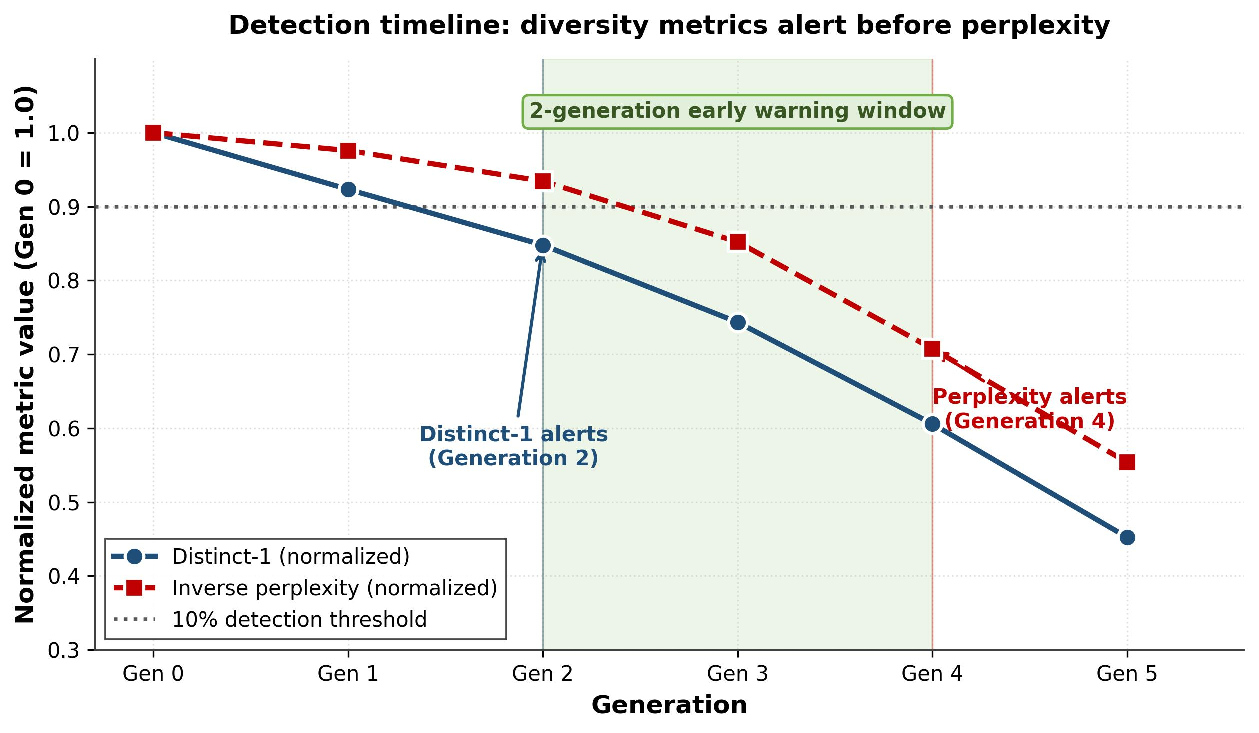
\includegraphics[width=0.92\textwidth]{figure1}
\caption{Detection timeline (GPT-2, replace scenario). \dist{1} crosses the 10\%
threshold at Generation~2; inverse perplexity crosses at Generation~4. The shaded
region marks the two-generation early-warning window. Values are normalized to
Generation~0.}
\label{fig:timeline}
\end{figure}

\subsection{Threshold Sensitivity Analysis}\label{sec:sensitivity}
Table~\ref{tab:sensitivity} shows detection timing across thresholds.

\begin{table}[t]
\centering
\caption{Threshold sensitivity: detection generation (GPT-2)}
\label{tab:sensitivity}
\begin{tabular}{lllll}
\hline\noalign{\smallskip}
Threshold & \dist{1} det. & PPL det. & Lead & False$+$ \\
\noalign{\smallskip}\hline\noalign{\smallskip}
5\%  & Gen 1 & Gen 3 & $+2$ & High      \\
10\% & Gen 2 & Gen 4 & $+2$ & Low       \\
15\% & Gen 2 & Gen 4 & $+2$ & Very low  \\
20\% & Gen 3 & Gen 5 & $+2$ & Minimal   \\
\noalign{\smallskip}\hline
\end{tabular}
\end{table}

\noindent\textbf{Key finding.} The two-generation lead time is robust across
thresholds from 5\% to 20\%. This is our central result: lead time is the
invariant, not the absolute threshold. The 10\% threshold is recommended as a
practical starting point, but organizations should calibrate to their baseline
variance. The ordering---diversity before perplexity---is the reliable signal.

\subsection{Mixed Scenario (30\% Synthetic)}
At 30\% synthetic, detection is slower, but the two-generation lead persists
(Generation~4 vs.\ Generation~6).

\begin{table}[t]
\centering
\caption{GPT-2: mixed scenario (30\% synthetic)}
\label{tab:mixed}
\begin{tabular}{ccccc}
\hline\noalign{\smallskip}
Gen & \dist{1} & PPL & $\Delta$\dist{1} & $\Delta$PPL \\
\noalign{\smallskip}\hline\noalign{\smallskip}
0 & .756 & 24.2 & --      & --      \\
2 & .712 & 24.5 & $-6\%$  & $+1\%$  \\
4 & .681 & 25.1 & $-10\%$ & $+4\%$  \\
6 & .634 & 26.8 & $-16\%$ & $+11\%$ \\
8 & .589 & 29.2 & $-22\%$ & $+21\%$ \\
\noalign{\smallskip}\hline
\end{tabular}
\end{table}

\subsection{Quantified Text Degradation}
Table~\ref{tab:degradation} shows the degradation pattern with concrete metrics.
Vocabulary contracts from 847 to 156 unique tokens (an 82\% reduction); repetition
rises from 12\% to 71\%. Rare technical terms such as ``glycolysis'' disappear by
Generation~3.

\begin{table}[t]
\centering
\caption{Text-quality degradation (GPT-2, 50 samples)}
\label{tab:degradation}
\begin{tabular}{cccl}
\hline\noalign{\smallskip}
Gen & Vocab size & Repetition \% & Example \\
\noalign{\smallskip}\hline\noalign{\smallskip}
0 & 847 & 12\% & ``\dots glycolysis, citric acid \dots'' \\
3 & 412 & 34\% & ``\dots important process \dots'' \\
5 & 156 & 71\% & ``\dots the the process \dots'' \\
\noalign{\smallskip}\hline
\end{tabular}
\end{table}

% =================================================================
\section{Discussion}\label{sec:discussion}

\subsection{Reversibility of Collapse}
Early detection (Generation~2--3) is fully reversible via checkpoint rollback. Late
detection (Generation~4) is partially reversible, requiring extended retraining,
and some vocabulary may not recover. Severe collapse (Generation~5 and beyond) is
effectively irreversible, requiring full retraining from scratch. Our
two-generation warning marks the boundary between reversible and irreversible
collapse.

\subsection{Why Diversity Metrics Detect First}
The consistent two-generation lead has a theoretical explanation grounded in the
``Tale of Tails'' framework~\cite{dohmatob2024tale}. Perplexity measures average
prediction quality across all tokens; this expectation is dominated by
high-frequency tokens and common patterns, which remain stable during early
collapse. A model can therefore maintain low perplexity while losing significant
tail coverage. In contrast, diversity metrics directly measure the support of the
output distribution---precisely what erodes first during collapse. \dist{1} counts
unique tokens and TTR measures vocabulary utilization; both are sensitive to tail
erosion by construction. Since collapse proceeds outside-in (tails before modes),
diversity metrics are inherently earlier indicators than performance metrics.

\subsection{Metric Selection Guidance}
We recommend \dist{1} as the primary metric (best efficiency, two-generation lead),
TTR as a secondary metric (equivalent lead, simpler computation), and perplexity
for confirmation. Entropy provides only a one-generation lead and is more expensive,
making it less suitable for primary monitoring.

\subsection{Alternative Early-Warning Approaches}
Embedding-space drift requires access to model internals, has high overhead, and is
unsuitable for API-based systems. Self-BLEU shows comparable lead time to \dist{1}
but has $O(n^2)$ complexity versus \dist{1}'s $O(n)$. Learned detectors require
labeled data, generalization across model families, and ongoing maintenance.
Diversity metrics are, by comparison, theoretically grounded, computationally
minimal, and require no model-internals access.

\subsection{Practical Deployment Recommendations}
For organizations deploying LLMs in production we recommend: establish baselines by
recording \dist{1} at model release; monitor daily by sampling 100 generations and
computing \dist{1}; alert at a 10\% relative drop; act within two generations to
preserve the reversibility window; and preserve original data to enable the
accumulate strategy where feasible.

\subsection{Limitations}\label{sec:limitations}
\noindent\textbf{Corpus scale.} Our 10-sample seed corpus is the most significant
limitation of this work. Production corpora contain millions of samples, and
collapse dynamics may differ qualitatively at scale; the observed 10\% threshold and
two-generation lead are specific to our experimental setting. The principle---that
diversity metrics detect collapse before perplexity---should generalize based on
theoretical grounding, but quantitative values require recalibration. Practitioners
should validate the principle on a small-scale pilot, establish corpus-specific
baselines, and treat 10\% as a starting point.

\noindent\textbf{Domain scope.} Our experiments use short, factual educational
prose. Collapse dynamics may differ substantially in other domains: code
generation, where syntactic constraints may preserve structure longer than lexical
diversity; instruction following, where format compliance may mask content
degradation; long-form creative text, where discourse structure may degrade before
token-level diversity; and multilingual or dialogue settings. Our results are most
directly applicable to factual content generation, and domain-specific validation
is required before deployment elsewhere.

\noindent\textbf{Model scale.} Both models tested (355M and 8B) exhibit detection
at Generation~2 and perplexity crossing at Generation~4, with similar relative
degradation trajectories, suggesting the ordering is not an artifact of a single
scale. We did not test larger models (e.g., 70B); since statistical (sampling)
error rather than functional (capacity) error drives tail erosion, we expect the
ordering to persist at larger scales, but direct validation remains future work.

\noindent\textbf{Architecture and fine-tuning.} Experimental claims are scoped to
autoregressive language models; cross-architecture validation (diffusion models,
GANs, multimodal) remains future work. The LLaMA~3 experiments use parameter-efficient
fine-tuning (QLoRA); full fine-tuning may exhibit quantitatively different dynamics,
though the qualitative pattern---diversity leads perplexity---should hold.

% =================================================================
\section{Related Work}\label{sec:related}
\noindent\textbf{Model collapse discovery.} Shumailov et
al.~\cite{shumailov2024nature} first demonstrated model collapse, showing
progressive degradation in OPT-125M over nine generations of recursive training, and
identified the mechanism: models lose information about the tails of the original
distribution. Alemohammad et al.~\cite{alemohammad2024mad} extended this to
diffusion models, documenting Model Autophagy Disorder.

\noindent\textbf{Theoretical foundations.} Dohmatob et
al.~\cite{dohmatob2025strong} proved that the collapse rate scales with the fraction
of synthetic data; their related ``Tale of Tails''
analysis~\cite{dohmatob2024tale}---that rare patterns erode first due to sampling
variance---directly motivates our use of diversity metrics as early-warning signals.

\noindent\textbf{Collapse prevention.} Gerstgrasser et
al.~\cite{gerstgrasser2024inevitable} proved that the accumulate strategy prevents
collapse entirely, a simple mitigation that nonetheless requires data storage and
provenance tracking.

\noindent\textbf{Definitional challenges and detection.} Schaeffer et
al.~\cite{schaeffer2025position} identified eight distinct definitions of model
collapse, motivating our reconciliation and operational criteria. Prior work has
focused primarily on documenting collapse rather than detecting it early; our
contribution fills this gap by systematically comparing detection metrics and
establishing lead times with statistical rigor.

\noindent\textbf{Efficient fine-tuning.} LoRA and its 4-bit extension QLoRA
\cite{dettmers2023qlora} enable parameter-efficient adaptation; we employ QLoRA to
make LLaMA~3-8B experiments computationally feasible while approximating full
fine-tuning behavior.

% =================================================================
\section{Conclusion}\label{sec:conclusion}
This paper establishes one principle for early detection of model collapse:
\emph{diversity metrics detect collapse before perplexity}. Our central
contribution is not a specific threshold (10\%) or lead time (2 generations) but the
robust ordering, which held across every condition we tested: threshold values from
5\% to 20\%, model scales from 355M to 8B parameters, contamination levels from 30\%
to 100\% synthetic, and against a Self-BLEU baseline. The theoretical basis is
clear: collapse proceeds outside-in, and diversity metrics directly measure tail
coverage while perplexity averages over all tokens.

Practitioners should adopt lightweight diversity monitoring (\dist{1}), establish
their own baselines rather than relying on our specific threshold, map generations
to their retraining cadence, and validate before production---our factual-prose
results may not transfer directly to code or instruction-following. We acknowledge
the principal limitations of corpus scale, domain coverage, and threshold
portability, and identify production-scale validation, domain-specific studies, and
cross-architecture validation as the foremost directions for future work.

\subsubsection*{Acknowledgments.} Experiments were conducted on Google Colab Pro
(NVIDIA A100). The author thanks the anonymous reviewers for their constructive
feedback.

% =================================================================
% ---- Bibliography ----
% References are listed in order of first citation in the text.
% NOTE: An inline thebibliography block is used so the file compiles
% without the external Springer .bst. If you prefer BibTeX, the
% accompanying references.bib is provided; switch to:
%     \bibliographystyle{splncs04}
%     \bibliography{references}
% (splncs04.bst ships with the Springer LNCS LaTeX package / Overleaf).
\begin{thebibliography}{10}

\bibitem{shumailov2024nature}
Shumailov, I., Shumaylov, Z., Zhao, Y., Papernot, N., Anderson, R., Gal, Y.:
AI models collapse when trained on recursively generated data. Nature \textbf{631},
755--759 (2024)

\bibitem{shumailov2023curse}
Shumailov, I., Shumaylov, Z., Zhao, Y., Gal, Y., Papernot, N., Anderson, R.:
The curse of recursion: training on generated data makes models forget.
arXiv:2305.17493 (2023)

\bibitem{schaeffer2025position}
Schaeffer, R., Kazdan, J., Arulandu, A.C., Koyejo, S.: Position: model collapse
does not mean what you think. arXiv:2503.03150 (2025)

\bibitem{dohmatob2024tale}
Dohmatob, E., Feng, Y., Yang, P., Charton, F., Kempe, J.: A tale of tails: model
collapse as a change of scaling laws. In: Proceedings of the 41st International
Conference on Machine Learning (ICML). Proceedings of Machine Learning Research,
vol. 235, pp. 11165--11197 (2024)

\bibitem{dohmatob2025strong}
Dohmatob, E., Feng, Y., Subramonian, A., Kempe, J.: Strong model collapse. In:
International Conference on Learning Representations (ICLR) (2025)

\bibitem{gerstgrasser2024inevitable}
Gerstgrasser, M., Schaeffer, R., Dey, A., Rafailov, R., Sleight, H., Hughes, J.,
Korbak, T., Agrawal, R., Pai, D., Gromov, A., Roberts, D.A., Yang, D., Donoho, D.L.,
Koyejo, S.: Is model collapse inevitable? Breaking the curse of recursion by
accumulating real and synthetic data. In: Conference on Language Modeling (COLM)
(2024)

\bibitem{meta2024llama3}
Meta AI: Llama 3 Model Card (2024), \url{https://github.com/meta-llama/llama3}

\bibitem{dettmers2023qlora}
Dettmers, T., Pagnoni, A., Holtzman, A., Zettlemoyer, L.: QLoRA: efficient
finetuning of quantized LLMs. In: Advances in Neural Information Processing Systems
(NeurIPS) (2023)

\bibitem{radford2019language}
Radford, A., Wu, J., Child, R., Luan, D., Amodei, D., Sutskever, I.: Language models
are unsupervised multitask learners. OpenAI Technical Report (2019)

\bibitem{alemohammad2024mad}
Alemohammad, S., Casco-Rodriguez, J., Luzi, L., Humayun, A.I., Babaei, H.,
LeJeune, D., Siahkoohi, A., Baraniuk, R.G.: Self-consuming generative models go MAD.
In: International Conference on Learning Representations (ICLR) (2024)

\end{thebibliography}

\end{document}
